%\documentclass{article}
%\usepackage{graphicx,subfigure}
%\begin{document}

\begin{figure}[!h]
  \centering
  \captionsetup{width=0.7\textwidth}
  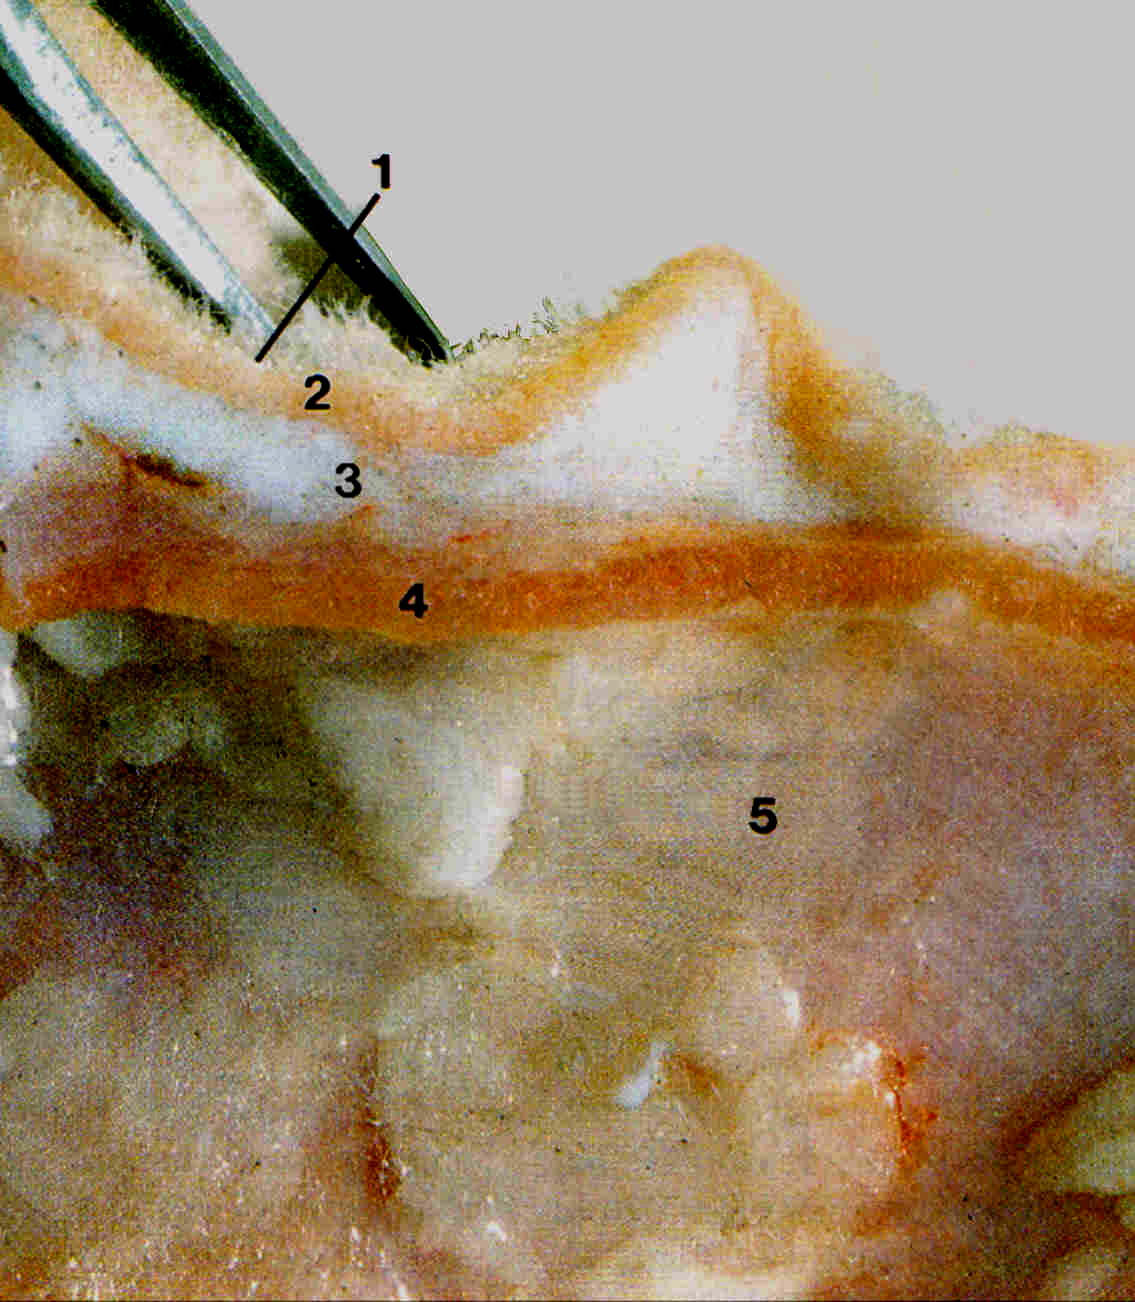
\includegraphics[width=0.7\textwidth]{mitchell.png}
  \caption{Merino sheep skin showing tissue layers. 1. epidermis with wool fibres; 2. papillary layer of dermis; 3. reticular layer of dermis; 4. areolar tissue and muscle; and 5. adipose tissue. One wrinkle is present on the right-hand side of the forceps. Forceps opening is $5 mm$. Modified from \citep{mitchell-1984}.}
  \label{fig:mitchell}
\end{figure}

%\end{document}

